\section{Army's Paeon}

The Repertoire buff from Army's Paeon is somewhat unique as it grants stacks of haste; each Repertoire stack grants one stack of a 4\% haste buff up to 12\% (a maximum of 4 stacks). The total number of GCDs during this window can vary due to how long it takes to reach the maximum haste strength. Formally, this results in the rotation itself becoming randomly distributed due differences in when exactly GCDs are executed.  From a damage variability perspective, we are only interested in how much the GCD count during Army's Paeon varies due to differences of when Repertoire procs occur. The damage distribution for a variable GCD count $c$ is

\begin{equation}
    P(D_{gcd}) = \sum_{i \in \{c\}}P_{gcd}(c=i) P(D; n=i)
    \label{eqn:ap-dmg-dist}
\end{equation}

Where $P_{gcd}$ is the probability that the haste buff results in a GCD count of $c$.\footnote{Accounting for Refulgent Arrow procs will be discussed later.} A 3-6-9 song sequence is assumed for computing $P_{gcd}$, as this sets the duration of Army's Paeon. For the first set of song sequences, Army's Paeon persists for 27 seconds and 9 Repertoire procs are possible. Empyreal Arrow is also used before Army's Paeon. For all subsequent song sequences, Army's Paeon persists for 36 seconds and 12 Repertoire procs are possible. Empyreal Arrow is used after Army's Paeon, immediately granting one stack of haste.

Modeling the number of GCDs analytically is incredibly complicated, as it depends on accounting for when exactly Repertoire procs are granted and how that affects future GCD lengths. Instead, the probability of achieving different GCD counts is simulated. Results are shown in Figure \ref{fig:ap-gcd-var}.

\begin{figure}[H]
    \centering
    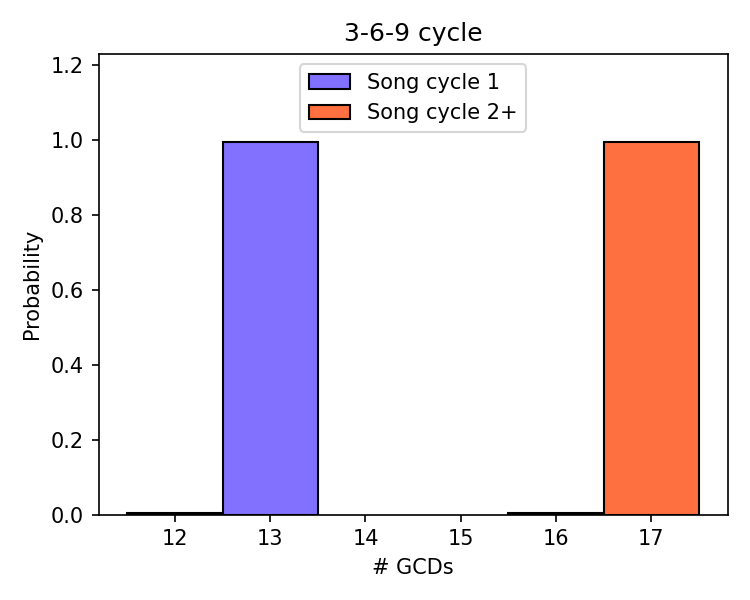
\includegraphics[scale=0.6]{img/ap-gcd-var.png}
    \caption{Probability of different GCD counts in Army's Paeon for a 3-6-9 song cycle for the first cycle (blue) and second cycle and beyond (orange).}
    \label{fig:ap-gcd-var}
\end{figure}

Somewhat surprisingly, there is effectively no variability in the GCD count and eqn. \ref{eqn:ap-dmg-dist} is entirely unneeded for this specific timing. It should be noted that for different durations of Army's Paeon, like 33 seconds, the probability of two different GCD counts being equally likely was also observed. This is probably because that time duration is near a boundary where an extra GCD would be granted.

Precisely sequencing actions with high fidelity, accounting for factors like application delay, animation lock, etc, is outside the scope of this paper, so it is not explored further.\footnote{Auto-attack count variability is ignored for the same reason. Note auto-attacks only deal 80 potency of damage.} Whether an extra GCD is negligible or not will require accounting for buff and action sequencing aspects like Army's Paeon duration, Empyreal Arrow timing, clipping, lag, minor drifting, etc with great care.

